% Chapter 2: Related Works
\section{A Low-Complexity and Adaptive DSC design for model aggregation in Distributed Learning  \cite{ZhangTao2022}}
this paper proposes a pipline for distributed compression of gradients for distributed learning. It tackles the aggregation bottleneck with a Wyner–Ziv–style DSC pipeline—quantization, Slepian–Wolf coding, and linear estimation—paired with an adaptive server “helper” that estimates gradient statistics, selects rates, and computes LLRs each round. In implementation, the method supports standard quantizers (e.g., multi-bit uniform and the 1-bit \emph{sign} scheme), partitions the full gradient vector into fixed-length blocks, and encodes them \emph{bit-plane by bit-plane}. Each bit-plane is Slepian–Wolf coded using \emph{LDPC syndrome} encoding at the workers, while the server performs \emph{successive decoding} that leverages previously decoded \emph{planes} and workers as side information, then linearly fuses the reconstructed blocks into the global update. The design is low-complexity, scales with the number of workers, and in experiments cuts communication substantially without harming accuracy—especially early in training when gradients are more correlated.
They also show that they can achive the rate limit set by the Slepian-Wolf theorem with the proposed scheme. results evaluated on MNIST, CIFAR-10, and SVHN, the method preserves accuracy (LDPC decoding BER <1\%) while cutting communication: e.g., SignSGD with their DSC saves ~38\% (MLP), 47\% (ResNet-20), and 37\% (ResNet-56) total communication; the gain is largest early in training when gradient correlation is stronger and shrinks as models converge.

\figure[htbp]
    \centering
    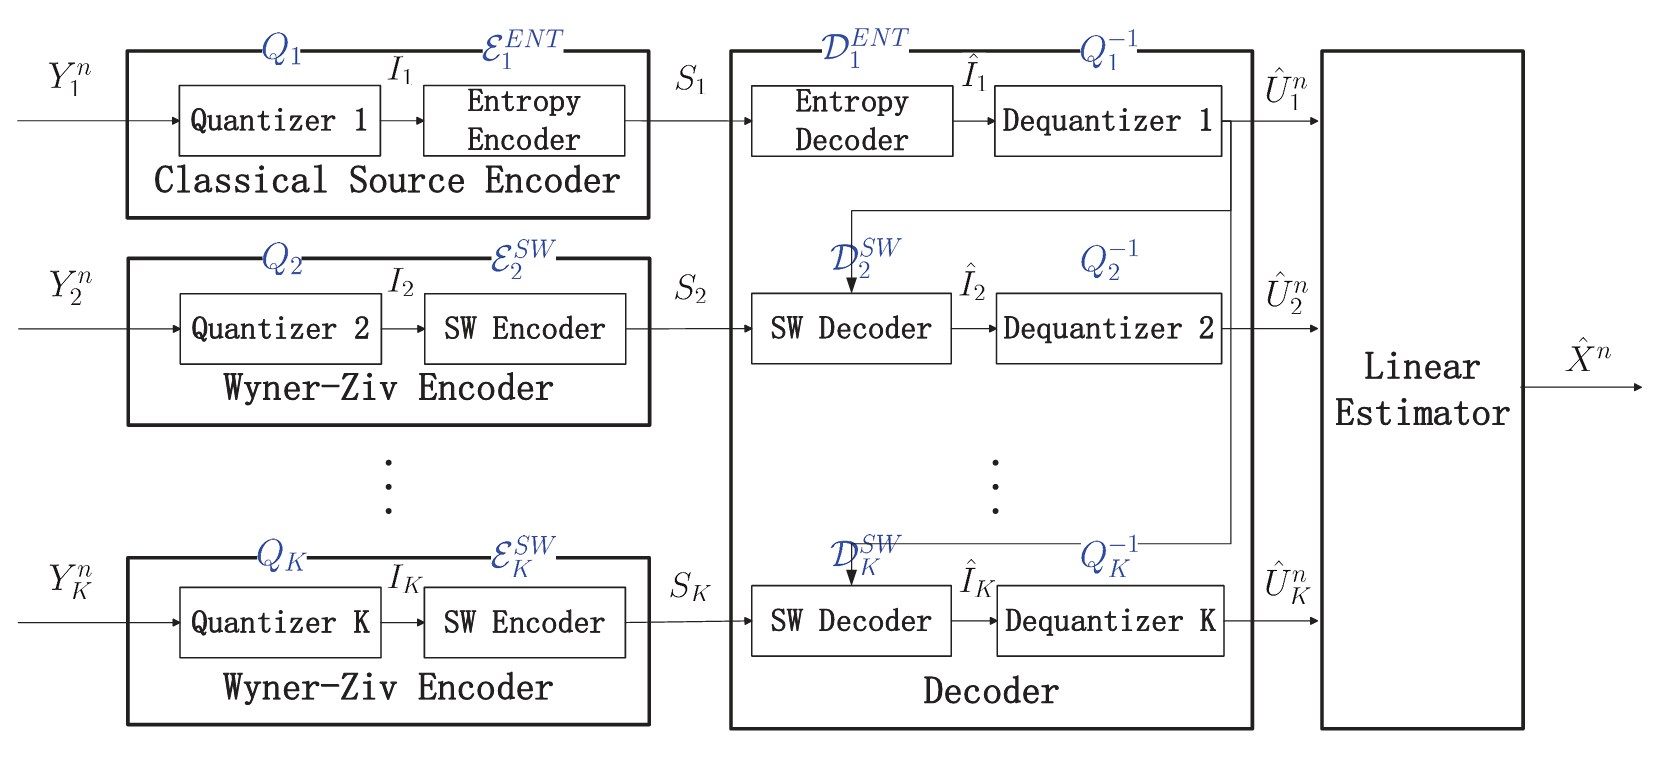
\includegraphics[width=0.8\textwidth]{Chapters/chapter_2_related_works/figures/zhangtao_DSC_pipeline}
    \caption{Pipeline of the proposed DSC scheme for distributed learning \cite{ZhangTao2022}.}
    \label{fig:DSC_pipeline}
\endfigure
